\documentclass[notitlepage]{revtex4-1}
\usepackage{geometry}
\usepackage{graphicx}
\usepackage{times}
\usepackage{physics}   % for simple physics notation
\usepackage{bm}        % for math
\usepackage{amssymb}   % for math
\usepackage{amsmath}
\usepackage{subfigure}
\usepackage{color}
\usepackage{float}
\usepackage{enumitem}
\usepackage[export]{adjustbox}
\usepackage{comment}
\usepackage{listings}
\usepackage{CJK}
\usepackage{graphicx}
\usepackage{booktabs}
\usepackage{hyperref}
\newcommand{\hilight}[1]{\colorbox{red}{#1}}
%\usepackage{physics}
%\usepackage{enumerate}
%\usepackage{booktabs} % not allowed in Revtex4.1
\begin{document}
\begin{CJK}{UTF8}{bsmi}
\title{First Principle 2017-Fall  Homework 3 Solution}
%\input author_list.tex       % D0 authors (remove the first 3 lines
                             % of this file prior to submission, they
                             % contain a time stamp for the authorlist)
                             % (includes institutions and visitors)
\author{Kai-Hsin Wu (吳愷訢)}
\email{r05222003@ntu.edu.tw}
\affiliation{Department of Physics and Center of Theoretical Sciences, National Taiwan University, Taipei 10607, Taiwan}

%\date{\today}
\maketitle

\begin{enumerate}	
	\item The following shows the result of Al and Na:
		\begin{itemize}
			\item Al
			\begin{enumerate}[label=(\arabic*)]
				\item $a_0$ using volume optimization:
				\begin{equation*}
					a_0 = 4.05000 \hspace{0.2cm} 
				\end{equation*}
				\item Variation with different $a_0$:
					\begin{center}
					\begin{tabular}{ c c }
						$a_0 (\AA)$ & $E (eV)$ \\ 
						3.90 &-14.541085 \\
						3.95 &-14.665726\\
						4.00  &-14.735369\\
						4.05 &-14.757538\\
						4.10  &-14.738699\\
						4.15 &-14.684395\\
						4.20  &-14.599834 
					\end{tabular}
					\end{center}
				
				\item the following figure shows the energy ($E$ ) v.s. $V$ :
					\begin{figure}[!h]
						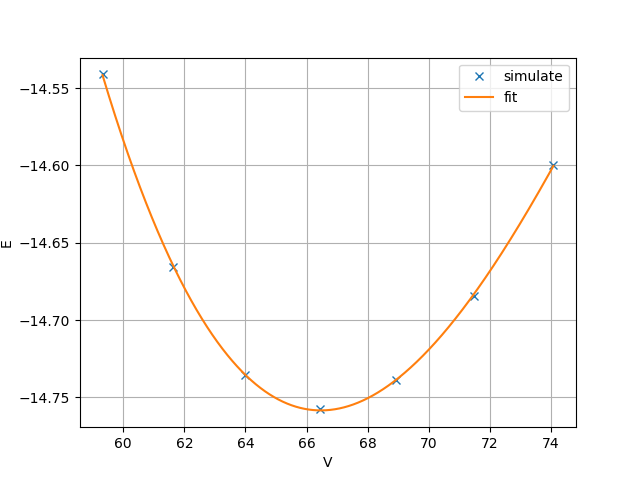
\includegraphics[width=8cm]{{Material/q1/Al_E-V}.png}
						\caption{Al-fcc E-V}
						\label{fig:AlE-V}
					\end{figure}
					
					By using third order polyfit, and with the following formula, we can get the bulk-modulus $B$ and the minimum $a_0$:
					\begin{align*}
					B &= V\frac{\partial^2}{\partial V^2} E \\
					V &= a_0^3
					\end{align*}
					\begin{align*}
					a_{0} &= 4.050723 \hspace{0.2cm} \AA\\
					B  &= 74.608739 \hspace{0.2cm} GPa
					\end{align*}
				
				\item  Consider the free electron HF energy density and seek for the minimum of $r_s$ :
				\begin{align*}
					e^{HF} &= \frac{A}{r_s^2} - \frac{\beta}{r_s} \\
					A &= 2.21 \\
					B &= 0.916
				\end{align*}
				Where the unit of energy is $Ry$ and $r_s$ is in unit of bohr radius ($bohr$). The minimum is at :
				\begin{equation*}
					r_s^{*} =\frac{2A}{\beta} (bohr)=  2.553467 \hspace{0.2cm} \AA 
				\end{equation*} 
				using following relation by which we consider 4 free electrons per unit-cell, we can estimate the lattice constant $a_0$ :
				\begin{align*}
					\frac{4\pi}{3}r_s^3 &= n^{-1} \\
					\frac{N_{free}}{a_0^3} &= n 
				\end{align*}
				
				\begin{align*}
					a_0 &= \left( \frac{16\pi}{3}\right)^{1/3} r_s \\
						&\approx 6.1737 \hspace{0.2cm} \AA \\
				\end{align*}
				
				For Bulk modulus, we have following relation. by which we express $\Omega$ in terms of $r_s$:
				\begin{align*}
					\frac{N}{\Omega} &= n = \frac{3}{4\pi r_s^3} \\
					B &= \Omega \frac{\partial^{2}E}{\partial \Omega^{2}} \\
					  &= \frac{1}{12\pi r_s}\left[ \frac{-2}{r_s}e^{HF'} + e^{HF''} \right] \\
					  &= \frac{1}{6\pi r_s^4} \left[ \frac{5A}{r_s} - 2\beta \right] \\
				\end{align*}

				we have the bulk modulus at $r_s^{*}$
				\begin{align*}
				B &= \frac{\beta^4}{6\pi(2A)^4} \frac{\beta}{2} (Ry/bohr^3)\\
				  &\approx 18.468 GPa
				\end{align*}
				
			\end{enumerate}
			\item Na
			%==================================================================
			\begin{enumerate}[label=(\arabic*)]
				\item $a_0$ using volume optimization:
				\begin{equation*}
				a_0 = 4.04669 \hspace{0.2cm} 
				\end{equation*}
				\item Variation with different $a_0$:
				\begin{center}
					\begin{tabular}{ c c }
						$a_0 (\AA)$ & $E (eV)$ \\ 
						3.9241059 &-1.437731 \\
						3.9645606 &-1.443730 \\
						4.0050153 &-1.447706 \\
						4.0454700 &-1.449866 \\
						4.0859247 &-1.449972 \\
						4.1263794 &-1.448133 \\
						4.1668341 &-1.445039 \\
						4.2072888 &-1.440498 
					\end{tabular}
				\end{center}
				
				\item the following figure shows the energy ($E$ ) v.s. $V$ :
				\begin{figure}[!h]
					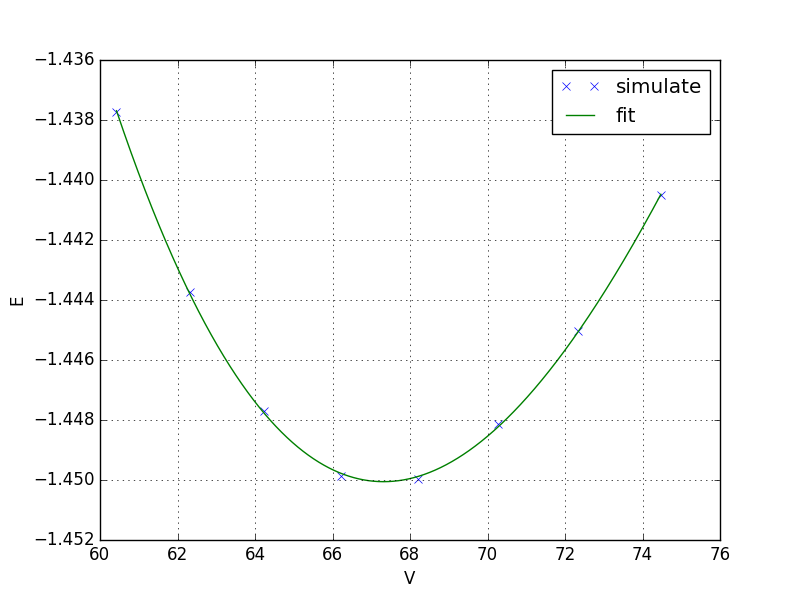
\includegraphics[width=8cm]{{Material/q1/Na_E-V}.png}
					\caption{Na-fcc E-V}
					\label{fig:NaE-V}
				\end{figure}
				
				By using third order polyfit, and with the following formula, we can get the bulk-modulus $B$ and the minimum $a_0$:
				\begin{align*}
				B &= V\frac{\partial^2}{\partial V^2} E \\
				V &= a_0^3
				\end{align*}
				\begin{align*}
				a_{0} &= 4.06802437 \hspace{0.2cm} \AA\\
				B  &= 4.83347453  \hspace{0.2cm} GPa 
				\end{align*}
				
				\item  Consider the free electron HF energy density and seek for the minimum of $r_s$ :
				\begin{align*}
				e^{HF} &= \frac{A}{r_s^2} - \frac{\beta}{r_s} \\
				A &= 2.21 \\
				B &= 0.916
				\end{align*}
				Where the unit of energy is $Ry$ and $r_s$ is in unit of bohr radius ($bohr$). The minimum is at :
				\begin{equation*}
				r_s^{*} =\frac{2A}{\beta} (bohr)=  2.553467 \hspace{0.2cm} \AA 
				\end{equation*} 
				using following relation by which we consider 2 free electrons per unit-cell, we can estimate the lattice constant $a_0$ :
				\begin{align*}
				\frac{4\pi}{3}r_s^3 &= n^{-1} \\
				\frac{N_{free}}{a_0^3} &= n 
				\end{align*}
				
				\begin{align*}
				a_0 &= \left( \frac{8\pi}{3}\right)^{1/3} r_s \\
				&\approx 5.186047 \hspace{0.2cm} \AA \\
				\end{align*}
				
				For Bulk modulus, we have following relation. by which we express $\Omega$ in terms of $r_s$:
				\begin{align*}
				\frac{N}{\Omega} &= n = \frac{3}{4\pi r_s^3} \\
				B &= \Omega \frac{\partial^{2}E}{\partial \Omega^{2}} \\
				&= \frac{1}{12\pi r_s}\left[ \frac{-2}{r_s}e^{HF'} + e^{HF''} \right] \\
				&= \frac{1}{6\pi r_s^4} \left[ \frac{5A}{r_s} - 2\beta \right] \\
				\end{align*}
				
				we have the bulk modulus at $r_s^{*}$
				\begin{align*}
				B &= \frac{\beta^4}{6\pi(2A)^4} \frac{\beta}{2} (Ry/bohr^3)\\
				&\approx 18.468 GPa
				\end{align*}
				
			\end{enumerate}	
		\end{itemize}
	\item For bcc Fe , doing LDA and GGA method with FM and NM :
		\begin{itemize}
			\item LDA 
				\begin{enumerate}[label=(\arabic*)]
					\item $a_0$ using volumn optimization :
					\begin{align*}
					a^{FM}_0 &=  2.744294 \hspace{0.2cm} \AA \\ 
					a^{NM}_0 &=  2.694591 \hspace{0.2cm} \AA  
					\end{align*} 
					\item minimization energy with variated $a_0$ and are showed in figure below:
					
					\begin{center}
						\begin{tabular}{*5c}
							\multicolumn{2}{c}{FM} &{}& \multicolumn{2}{c}{NM} \\
							$a_0 (\AA)$   & $E (eV)$    &{}& $a_0 (\AA)$   & $E (eV)$\\
							2.60 &-8.967318 &{}&2.55 &-8.672935 \\
							2.65 &-9.121350 &{}&2.60 &-8.863644 \\
							2.70 &-9.206677 &{}&2.65 &-8.964152 \\
							2.75 &-9.228247 &{}&2.70 &-8.988743 \\
							2.80 &-9.202380 &{}&2.75 &-8.952579 \\ 
							2.85 &-9.135795 &{}&2.80 &-8.867398 \\
							2.90 &-9.048763 &{}&2.85 &-8.742378 \\
							2.95 &-8.935725	&{}&2.90 &-8.585827
						\end{tabular}			

						\begin{figure}[!h]
							\centering
								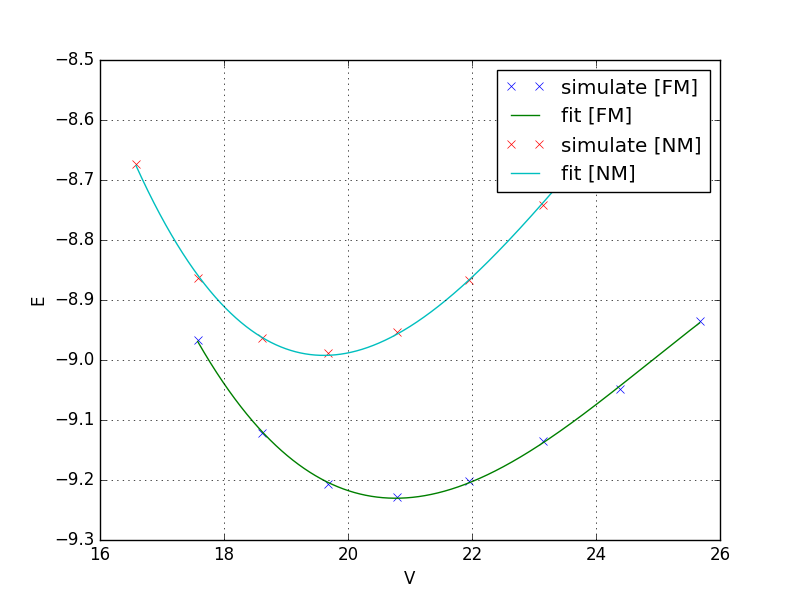
\includegraphics[width=10cm]{{Material/q2/LDA_E-V-FMNM}.png}
							\caption{Fe-bcc LDA E-V}
							\label{fig:LDAFeE-VFMNM}
						\end{figure}
					\end{center}
					The minimized $a_0$ and $B$ of bcc Fe with FM and NM are :
					\begin{align*}
					a_0^{FM} &=	 2.746787 \AA \hspace{0.5cm} &B^{FM} &=  134.99746 GPa \\
					a_0^{NM} &=  2.694740 \AA \hspace{0.5cm} &B^{NM} &=  175.45431 GPa \\
					\end{align*} 
					
					We see that the FM case has minimal energy, which shows the ground state is Ferromagnetic. 
				\end{enumerate}
			\newpage
			\item GGA 
				\begin{enumerate}[label=(\arabic*)]
					\item $a_0$ using volumn optimization :
						\begin{align*}
							a^{FM}_0 &= 2.82214 \hspace{0.2cm} \AA \\ 
							a^{NM}_0 &= 2.75412 \hspace{0.2cm} \AA  
						\end{align*} 
					\item minimization energy with variated $a_0$ and are showed in figure below:
						
						\begin{center}
							\begin{tabular}{*5c}
								 \multicolumn{2}{c}{FM} &{}& \multicolumn{2}{c}{NM} \\
								 $a_0 (\AA)$   & $E (eV)$    &{}& $a_0 (\AA)$   & $E (eV)$\\
								 2.70 &-8.009989 &{}&2.70 &-7.724527 \\
								 2.75 &-8.108553 &{}&2.75 &-7.757336 \\
								 2.80 &-8.151154 &{}&2.80 &-7.737622 \\
								 2.85 &-8.158445 &{}&2.85 &-7.674045 \\
								 2.90 &-8.135495 &{}&2.90 &-7.575350 \\ 
								 2.95 &-8.077445 &{}&2.95 &-7.448175 \\
								 3.00 &-8.000995 &{}&3.00 &-7.298845
							\end{tabular}			
						
							\begin{figure}[!h]
								\centering
								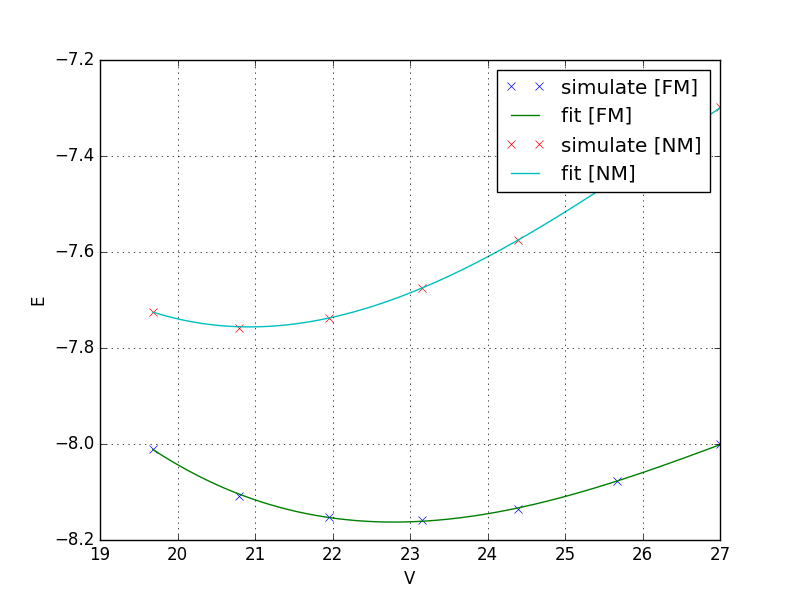
\includegraphics[width=10cm]{{Material/q2/GGA_E-V-FMNM}.png}
								\caption{Fe-bcc GGA E-V}
								\label{fig:GGAFeE-VFMNM}
							\end{figure}
						\end{center}
					The minimized $a_0$ and $B$ of bcc Fe with FM and NM are :
					\begin{align*}
						a_0^{FM} &=	2.834269 \AA \hspace{0.5cm} &B^{FM} &= 93.907626 GPa \\
						a_0^{NM} &= 2.755061 \AA \hspace{0.5cm} &B^{NM} &= 124.57160 GPa \\
					\end{align*} 
					
					We see that the FM case has minimal energy, which consist with the GGA results that the ground state is Ferromagnetic. 
					 
					
				\end{enumerate}
		\end{itemize}
	\item GGA band gaps of typical semiconductors, the following experiment value comes from \cite{Bandref} 
	\begin{itemize}
		\item Si
		\begin{enumerate}[label=(\arabic*)]
			\item $a_0$ using volumn optimization :
			\begin{align*}
			a^{Si}_0 &= 5.46078 \hspace{0.2cm} \AA 
			\end{align*} 
			\item The band structure and density of state are shown below :
			
			\begin{figure}[!h]
				\centering
				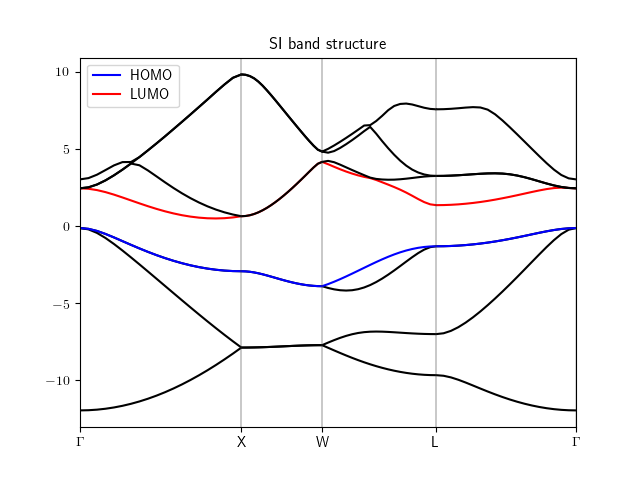
\includegraphics[width=10cm]{{Material/q3/si}.png}
				\caption{Si band-structure}
				\label{fig:Si-band}
			\end{figure}
			The band gap $E^{Si}_g$ is :
			\begin{align*}
				E^{Si}_g = 0.6245 \hspace{0.2cm}  eV
			\end{align*}
		
		
		\end{enumerate}
		\newpage
		\item Ge
		\begin{enumerate}[label=(\arabic*)]
			\item $a_0$ using volumn optimization :
			\begin{align*}
			a^{Ge}_0 &= 5.76822 \hspace{0.2cm} \AA 
			\end{align*} 
			\item The band structure and density of state are shown below :

			\begin{figure}[!h]
				\centering
				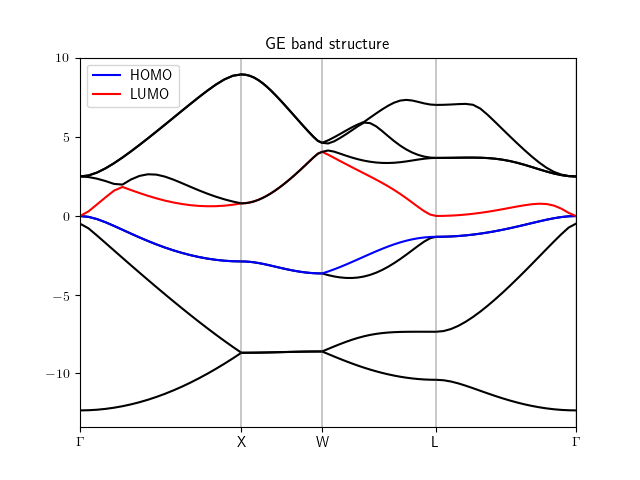
\includegraphics[width=10cm]{{Material/q3/Ge}.png}
				\caption{Ge band-structure}
				\label{fig:Ge-band}
			\end{figure}
				The band gap $E^{Ge}_g$ is :
				\begin{align*}
					E^{Ge}_g = 0.0 \hspace{0.2cm} eV
				\end{align*}
		\end{enumerate}

		\newpage
		\item GaAs
		\begin{enumerate}[label=(\arabic*)]
			\item $a_0$ using volumn optimization :
			\begin{align*}
			a^{GaAs}_0 &= 5.751291 \hspace{0.2cm} \AA 
			\end{align*} 
			\item The band structure and density of state are shown below :

				\begin{figure}[!h]
					\centering
					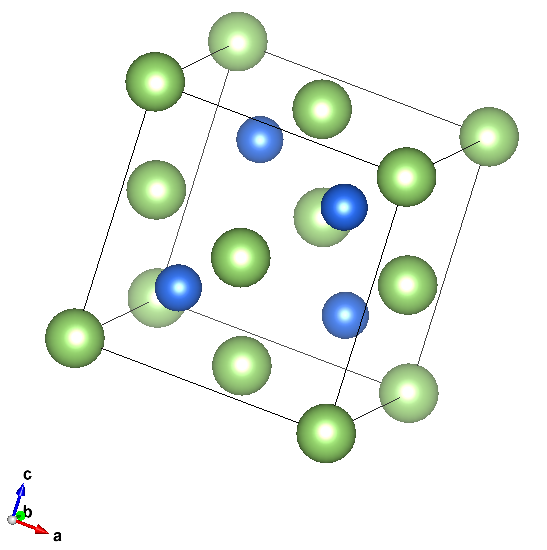
\includegraphics[width=10cm]{{Material/q3/GaAs}.png}
					\caption{GaAs band-structure}
					\label{fig:GaAs-band}
				\end{figure}
				The band gap $E^{GaAs}_g$ is :
				\begin{align*}
				E^{GaAs}_g = 0.1755 \hspace{0.2cm} eV
				\end{align*}
		\end{enumerate}		
	\end{itemize}
\end{enumerate}


\end{CJK}

\bibliographystyle{apsrev4-1}
\bibliography{ref}
	

\end{document}

